
  
 	 \section{Introduction}
 	  
    
    Le cloud computing, traduit le plus souvent en français par " informatique dans les nuages", " informatique dématérialisée " ou encore " infonuagique ", est un domaine qui regroupe un ensemble de techniques et de pratiques consistant à accéder, en libre-service, à du matériel ou à des logiciels informatiques, à travers une infrastructure réseau (Internet). Ce concept rend possible la distribution des ressources informatiques sous forme de services pour lesquels l'utilisateur paie uniquement pour ce qu'il utilise. Ces services peuvent être utilisés pour exécuter des applications scientifiques et commerciales, souvent modélisées sous forme de workflows.
     
    Ce chapitre présente une introduction au cloud computing et au workflow, nécessaire pour la compréhension générale de ce rapport.
    
    Tout d’abord, nous présentons dans la section 1.2 une introduction au paradigme du cloud computing. Nous donnons un aperçu général du cloud computing, y compris sa définition, ses caractéristiques principales et une comparaison avec les technologies connexes. Nous présentons les différents modèles de service, les différents modèles de déploiement, ainsi que les différents acteurs du cloud computing. Nous résumons quelques challenges de recherche en cloud computing. Par la suite, nous présentons, dans la section 1.3, une introduction au workflow et systèmes de gestion de workflow. Nous donnons le concept du workflow, sa définition, et l’architecture de référence d’un système de gestion de workflows. Nous énumérons quelques systèmes de gestion de workflows existant dans les grilles et clouds et, finalement, nous résumons l’intérêt  du cloud pour les workflows.
    
    \section{cloud computing}
    \subsection{Concept du cloud computing}
  L’idée principale du cloud est apparue dans les années 60, où le professeur John McCarthy avait imaginé que les ressources informatiques seront fournies comme des services d’utilité publique (Garfinkel, 1999). C'est ensuite, vers la fin des années 90, que ce concept a pris de l'importance avec l’avènement du grid computing  (Foster, 1999). Le terme cloud est une métaphore exprimant la similarité avec le réseau électrique, dans lequel l'électricité est produite dans de grandes centrales, puis disséminée à travers un réseau jusqu'aux utilisateurs finaux. Ici, les grandes centrales sont les Datacenter, le réseau est le plus souvent celui d'Internet et l'électricité correspond aux ressources informatiques. Le cloud computing  n'est véritablement apparu qu'au cours de l’année 2006 (Vouk, 2008) avec l'apparition d'Amazon EC2 (Elastic Compute cloud). C'est en 2009 que la réelle explosion du cloud survint avec l'arrivée sur le marché de sociétés comme Google (Google App Engine), Microsoft (Microsoft Azure), IBM (IBM Smart Business Service), Sun (Sun cloud) et Canonical Ltd (Ubuntu Enterprise cloud). D'après une étude menée par Forrester (Ried, 2011), le marché du cloud computing  s'élevait à environ 5,5 milliards de dollars en 2008, il devrait atteindre plus de 150 milliards d'ici 2020, comme l’illustre la figure \ref{fig:tempsnip4}. 
    
    \begin{figure}[h]
    	\centering
    	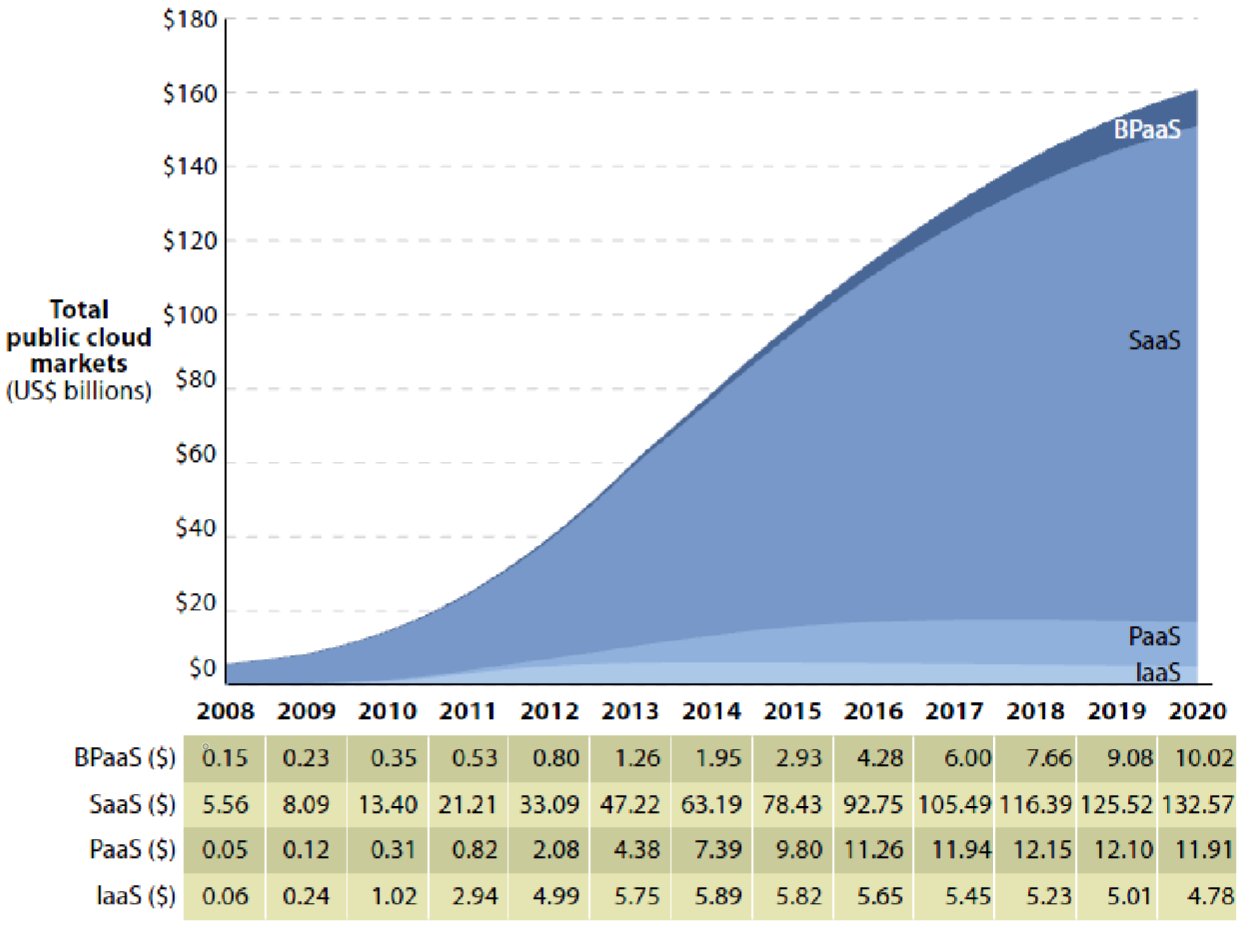
\includegraphics[width=0.7\linewidth]{images/tempsnip4}
    	\caption{Prévisions de la taille du marché du cloud computing  public (Ried, 2011).}
    	\label{fig:tempsnip4}
    \end{figure}
\subsubsection{Vers une définition du cloud computing }
Beaucoup de chercheurs ont tenté de définir le cloud computing (Geelan, 2008 ; McFedries, 2008 ; Buyya, 2009 ; Armbrust, 2010). La plupart des définitions attribuées à ce concept semblent se concentrer seulement sur certains aspects technologiques. L'absence d'une définition standard a généré non seulement des exagérations du marché, mais aussi des confusions. Pour cette raison, il y a eu récemment des travaux sur la normalisation de la définition du cloud computing, à l'exemple de Vaquero et coll (Vaquero, 2009) qui ont comparé plus de 20 définitions différentes et ont proposé une définition globale.  En guise de synthèse des différentes propositions données dans la littérature, nous introduisons une définition mixte, qui correspond aux différents types de cloud considérés dans les travaux réalisés dans cette thèse.

  Nous définissons le cloud comme un modèle informatique qui permet d’accéder, d’une façon transparente et à la demande, à un pool de ressources hétérogènes physiques ou virtualisées (serveurs, stockage, applications et services) à travers le réseau. Ces ressources sont délivrées sous forme de services reconfigurables et élastiques, à base d’un modèle de paiement à l’usage, dont les garanties sont offertes par le fournisseur via des contrats de niveau de service (SLA, Service Level Agreement).     
    
    \subsubsection{Caractéristiques principales du cloud computing}
    Le cloud computing  possède les caractéristiques suivantes :
    \begin{itemize}
    	\item 	\textbf{Accès en libre-service à la demande}. Le cloud computing offre des ressources et services aux utilisateurs à la demande. Les services sont fournis de façon automatique, sans nécessiter d’interaction humaine (Mell, 2011). 
    \item	\textbf{Accès réseau universel.}  Les services de cloud computing  sont facilement accessibles au travers du réseau, par le biais de mécanismes standard, qui permettent une utilisation depuis de multiples types de terminaux (par exemple, les ordinateur portables, tablettes, smartphones) (Mell, 2011). 
   \item \textbf{Mutualisation de ressources} (Pooling). Les ressources du cloud peuvent être regroupées pour servir des utilisateurs multiples, pour lesquels des ressources physiques et virtuelles sont automatiquement attribuées (Mell, 2011). En général, les utilisateurs n’ont aucun contrôle ou connaissance sur l’emplacement exact des ressources fournies. Toutefois, ils peuvent imposer de spécifier l’emplacement à un niveau d’abstraction plus haut.
   \item \textbf{Scalabilité et élasticité.} Des ressources supplémentaires peuvent être automatiquement mises à disposition des utilisateurs en cas d’accroissement de la demande (en réponse à l'augmentation des charges des applications) (Geelan, 2008), et peuvent être libérées lorsqu’elles ne sont plus nécessaires. L’utilisateur a l’illusion d’avoir accès à des ressources illimitées à n'importe quel moment, bien que le fournisseur en définisse généralement un seuil (par exemple : 20 instances par zone est le maximum possible pour Amazon EC2).
   \item \textbf{Autonome.} Le cloud computing  est un système autonome et géré de façon transparente pour les utilisateurs. Le matériel, le logiciel et les données au sein du cloud peuvent être 
    	automatiquement reconfigurés, orchestrés et consolidés en une seule image qui sera fournie à l’utilisateur (Wang, 2008).
    	\item \textbf{Paiement à l’usage.} La consommation des ressources dans le cloud s’adapte au plus près aux besoins de l’utilisateur. Le fournisseur est capable de mesurer de façon précise la consommation (en durée et en quantité) des différents services (CPU, stockage, bande passante,…) ; cela lui permettra de facturer l’utilisateur selon sa réelle consommation (Armbrust, 2009). 
    	\item \textbf{Fiabilité et tolérance aux pannes.} Les environnements cloud tirent parti de la redondance intégrée du grand nombre de serveurs qui les composent en permettant des niveaux élevés de disponibilité et de fiabilité pour les applications qui peuvent en bénéficier (Buyya, 2008). 
    	\item \textbf{Garantie QoS.} Les environnements de cloud peuvent garantir la qualité de service pour les utilisateurs, par exemple, la performance du matériel, comme la bande passante du processeur et la taille de la mémoire (Wang, 2008). 
    	\item \textbf{Basé-SLA.} Les clouds sont gérés dynamiquement en fonction des contrats d’accord de niveau de service (SLA) (Buyya, 2008) entre le fournisseur et l’utilisateur. Le SLA définit des politiques, telles que les paramètres de livraison, les niveaux de disponibilité, la maintenabilité, la performance, l'exploitation, ou autres attributs du service, comme la facturation, et même des sanctions en cas de violation du contrat. Le SLA permet de rassurer les utilisateurs dans leur idée de déplacer leurs activités vers le cloud, en fournissant des garanties de QoS. 
    	Après avoir présenté les caractéristiques essentielles d’un service cloud, nous présentons, brièvement, dans la section suivante, quelques technologies connexes aux clouds.
    	
    \end{itemize} 
\subsection{Technologies connexes }

\subsection{Modèles du cloud computing  }
\subsubsection {Modèles de service du cloudcomputing}  
XaaS (X as a Service) représente la base du paradigme du cloud computing, où X représente un service tel qu’un logiciel, une plateforme, une infrastructure, un Business Process, etc. Nous présentons, dans cette section,  quatre  modèles de services (Rimal, 2009), à savoir: (1) Logiciel en tant que services SaaS (Software as a Service), où le matériel, l’hébergement, le framework d’application et le logiciel sont dématérialisés, (2) Plateforme en tant que service PaaS (Platform as a Service), où le matériel, l’hébergement et le framework d’application sont dématérialisés, (3) Infrastructure en tant que service IaaS (Infrastructure as a Service) et (4) Matériel en tant que service HaaS (Hardware as a Service), où seul le matériel (serveurs) est dématérialisé dans ces deux derniers cas. La figure \ref{fig:capture5} montre le modèle classique et les différents modèles de service de cloud
\begin{figure}[h]
	\centering
	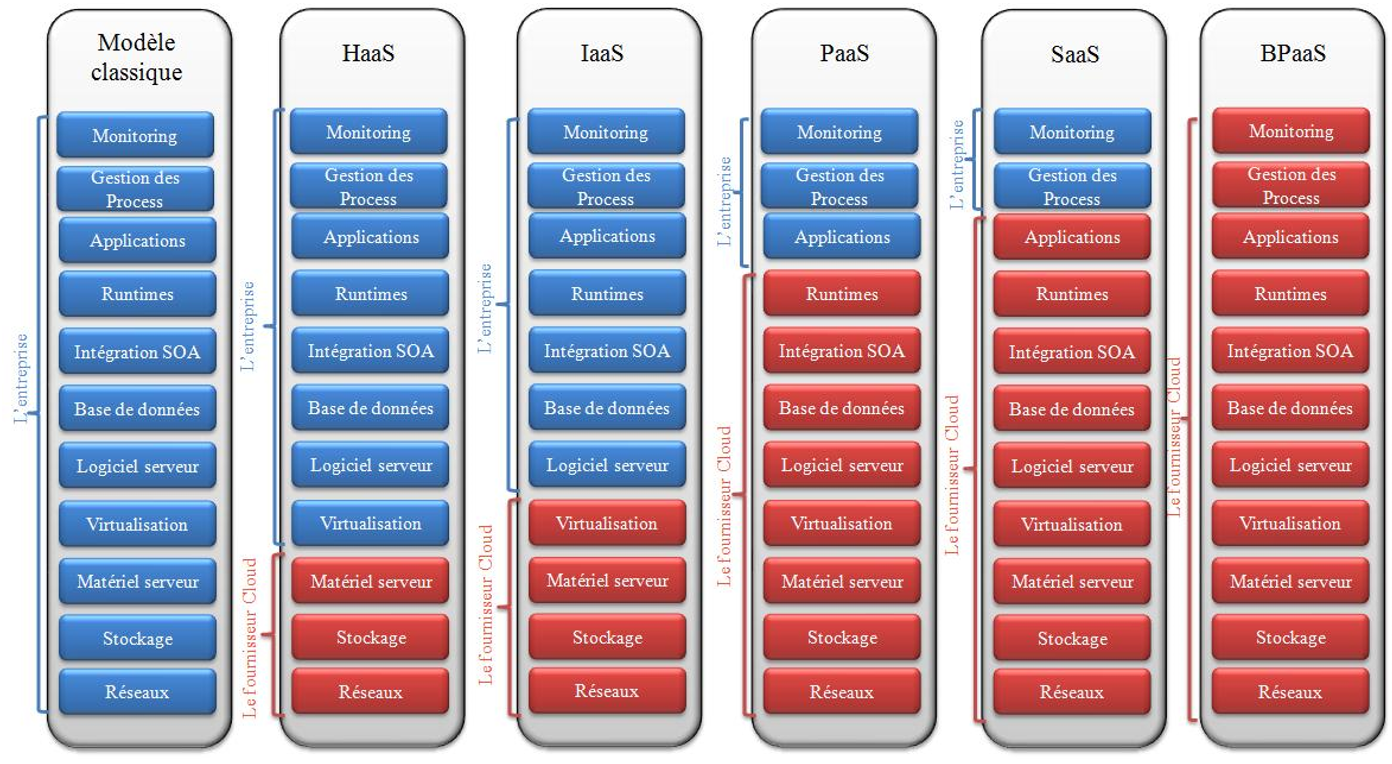
\includegraphics[width=0.7\linewidth]{Capture5}
	\caption{Les services XaaS du cloud computing}
	\label{fig:capture5}
\end{figure}

\begin{enumerate}
\item 	\textbf{Software as a Service (SaaS):}

Ce modèle de service est caractérisé par l’utilisation d’une application partagée qui fonctionne sur une infrastructure Cloud. L’utilisateur accède à l’application par le réseau au travers de divers types de terminaux (souvent via un navigateur web). L’administrateur de l’application ne gère pas et ne contrôle pas l’infrastructure sous-jacente (réseaux, serveurs, applications, stockage).  Il ne contrôle pas les fonctions de l’application à l’exception d’un paramétrage de quelques fonctions utilisateurs limitées. On prend comme exemple les logiciels de messagerie au travers d’un navigateur comme Gmail ou Yahoo mail. 

\item  \textbf{ Platform as a Service (PaaS):}

L’utilisateur a la possibilité de créer et de déployer sur une infrastructure Cloud PaaS ses propres applications en utilisant les langages et les outils du fournisseur. L’utilisateur ne gère pas ou ne contrôle pas l’infrastructure Cloud sous-jacente (réseaux, serveurs, stockage) mais l’utilisateur contrôle l’application déployée et sa configuration. Comme exemple de PaaS, on peut citer un des plus anciens -IntuitQuickbase- qui permet de déployer ses applications bases de données en ligne ou -Google Apps Engine (GAE)- pour déployer des services Web. 

Dans ces deux cas l’utilisateur de ces services n’a pas à gérer des serveurs ou des systèmes pour déployer ses applications en ligne et dimensionner des ressources adaptées au trafic.
\item   \textbf{Infrastructure as a Service (IaaS):}

L’utilisateur loue des moyens de calcul et de stockage, des capacités réseau et d’autres ressources indispensables (partage de charge, pare-feu, cache). L’utilisateur a la possibilité de déployer n’importe quel type de logiciel incluant les systèmes d’exploitation. L’utilisateur ne gère pas ou ne contrôle pas l’infrastructure Cloud sous-jacente mais il a le contrôle sur les systèmes d’exploitation, le stockage et les applications. Il peut aussi choisir les caractéristiques principales des équipements réseau comme le partage de charge, les pare-feu, etc. L’exemple emblématique de ce type de service est Amazon Web Services qui fournit du calcul (EC2), du stockage (S3, EBS), des bases de données en ligne (SimpleDB) et quantité d’autres services de base. Il est maintenant imité par de très nombreux fournisseurs.
	\item \textbf{Points fortset Points faibles des services cloud:} 
\end{enumerate}
\begin{table}[h]
	\begin{tabular}{l|l|l|ll}
		
		\cline{2-3}
		& Points forts                                                                                              & Points faibles                                                                                                                            &  &  \\ \cline{1-3}
		\multicolumn{1}{|l|}{SaaS} & \begin{tabular}[c]{@{}l@{}}Pas d’installation\\  Plus de licence\end{tabular}                             & \begin{tabular}[c]{@{}l@{}}Logiciel limité\\ Sécurité\\ Dépendance de prestataire\end{tabular}                                             \\ \cline{1-3}
		\multicolumn{1}{|l|}{PaaS} & \begin{tabular}[c]{@{}l@{}}Pas d'infrastructure Nécessaire\\ Pas d'infrastructure Nécessaire\end{tabular} & \begin{tabular}[c]{@{}l@{}}Limitation des langages\\ Pas de personnalisation dans la configuration des\\ machines virtuelles\end{tabular}   \\ \cline{1-3}
		\multicolumn{1}{|l|}{IaaS} & \begin{tabular}[c]{@{}l@{}}Administration\\  Personnalisation\\ Flexibilité d'utilisation\end{tabular}    & \begin{tabular}[c]{@{}l@{}}Sécurité\\ Besoin d'un administrateur système\end{tabular}                                                    \\ \cline{1-3}
	\end{tabular}
	
	
	
	\caption{Points forts et Points faibles des services Cloud}
	\label{tab:tabl1}
\end{table}
\subsubsection { Modèles de déploiement}  

Selon la définition du cloud computing  donnée part le NIST (Mell, 2011), il existe quatre modèles de déploiement des services de cloud, à savoir : cloud privé, cloud communautaire, cloud public et cloud hybride, comme illustré dans la figure \ref{fig:cloudmd}.
\begin{enumerate}
	\item \textbf{Cloud privé :}\\
	 L’ensemble des ressources d’un cloud privé est exclusivement mis à disposition d’une entreprise ou organisation unique. Le cloud privé peut être géré par l’entreprise ellemême (cloud privé interne) ou par une tierce partie (cloud privé externe). Les ressources d’un cloud privé se trouvent généralement dans les locaux de l’entreprise ou bien chez un fournisseur de services. Dans ce dernier cas, l’infrastructure est entièrement dédiée à l’entreprise et y est accessible via un réseau sécurisé (de type VPN).  L’utilisation d’un cloud privé permet de 	garantir, par exemple, que les ressources matérielles allouées ne seront jamais partagées par deux clients différents. 
	
	\item \textbf{Cloud communautaire:}\\
	 L’infrastructure d’un cloud communautaire est partagée par plusieurs organisations indépendantes ayant des intérêts communs. L’infrastructure peut être gérée par les organisations membres ou par un tiers. L’infrastructure peut être située, soit au sein des dites organisations, soit chez un fournisseur de services. 
	\item \textbf{Cloud public:}\\
	L’infrastructure d’un cloud public est accessible à un large public et appartient à un fournisseur de services. Ce dernier facture les utilisateurs selon la consommation et garantit la disponibilité des services via des contrats SLA. 
	\item \textbf{Cloud hybride:}\\
	 L’infrastructure d’un cloud hybride est une composition de plusieurs clouds (privé, communautaire ou public). Les différents clouds composant l’infrastructure restent des entités uniques, mais sont reliés par une technologie standard ou propriétaire permettant ainsi la portabilité des données ou des applications déployées sur les différents clouds.  

\begin{figure}[h]
	\centering
	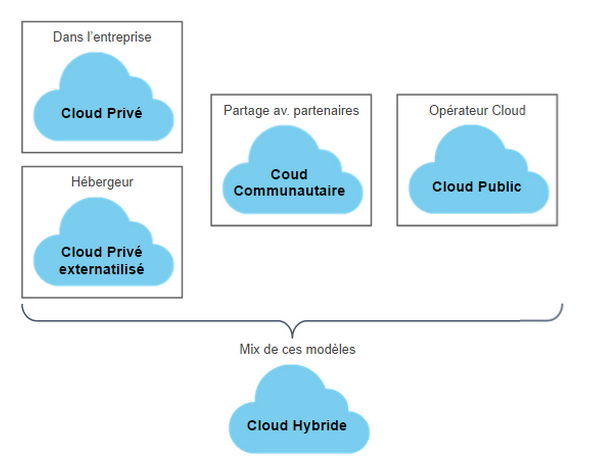
\includegraphics[width=0.5\linewidth]{Cloud_MD}
	\caption{Modèles de déploiement du cloud computing }
	\label{fig:cloudmd}
\end{figure}
\end{enumerate}



%%%%%%%%%%%%%%%%%%%%%%%%%%%%              Workflow et systèmes de gestion de workflows 
%%%%%%%%%%%%%%%%%%%%%%%%%%%%

 \section{Workflow et systèmes de gestion de Workflow}
 	 
 	 \subsection{ Concepts de base et définitions de Workflow }
 	 
 
La notion de workflow (traduit en français par "flux de travail") est apparue dans l’industrie de l’image électronique et de la gestion de production assistée par ordinateur (GW, 1998). Ce concept a donc été créé dans le but d’automatiser les procédures de travail au sein des organisations. L’idée d’enchaîner différentes tâches pour réaliser un traitement complexe est pertinente. De plus, dans les infrastructures actuelles distribuées, gérant des ressources hétérogènes, telles que le cloud computing, bénéficier d’un environnement autorisant la définition et l’exécution des chaînes de traitement constitue une des fonctionnalités essentielles recherchée, à la fois par les scientifiques et au-delà par le grand public.

Deux grandes catégories d’usages utilisent la notion de workflow : les protocoles expérimentaux, dans des domaines tels que la biologie, l’astronomie, la physique, la neuroscience, la chimie, etc. (workflows scientifiques) et les chaînes de traitement pratiquées dans des domaines commerciaux, financiers, pharmaceutiques (processus métiers). Elles donnent lieu à plusieurs pistes de recherche diverses, mais cependant connexes. Dans le cadre de cette thèse, nous traitons plus particulièrement les workflows scientifiques.

\subsubsection{Définitions de workflow}
La WfMC (Workflow Management Coalition) (WfMC, 1999) a donné une définition qui généralise la notion de workflow indépendamment des domaines spécifiques:

"Workflow is the automation of business process, in whole or part during which documents, information or tasks are passed from one participant to another for action, according to a set of procedural rules."

Nous traduisons cette définition par: " Un workflow est l'automatisation d'un processus métier, en tout ou en partie, au cours de laquelle des documents, des informations ou des tâches sont passées d'un participant à un autre pour l'action, selon un ensemble de règles procédurales". 

 	 
